\documentclass{mynote}

\title{Exercise1}
\author{202005100214}
\date\today


\begin{document}
\maketitle
\begin{figure}[H]
    \centering
    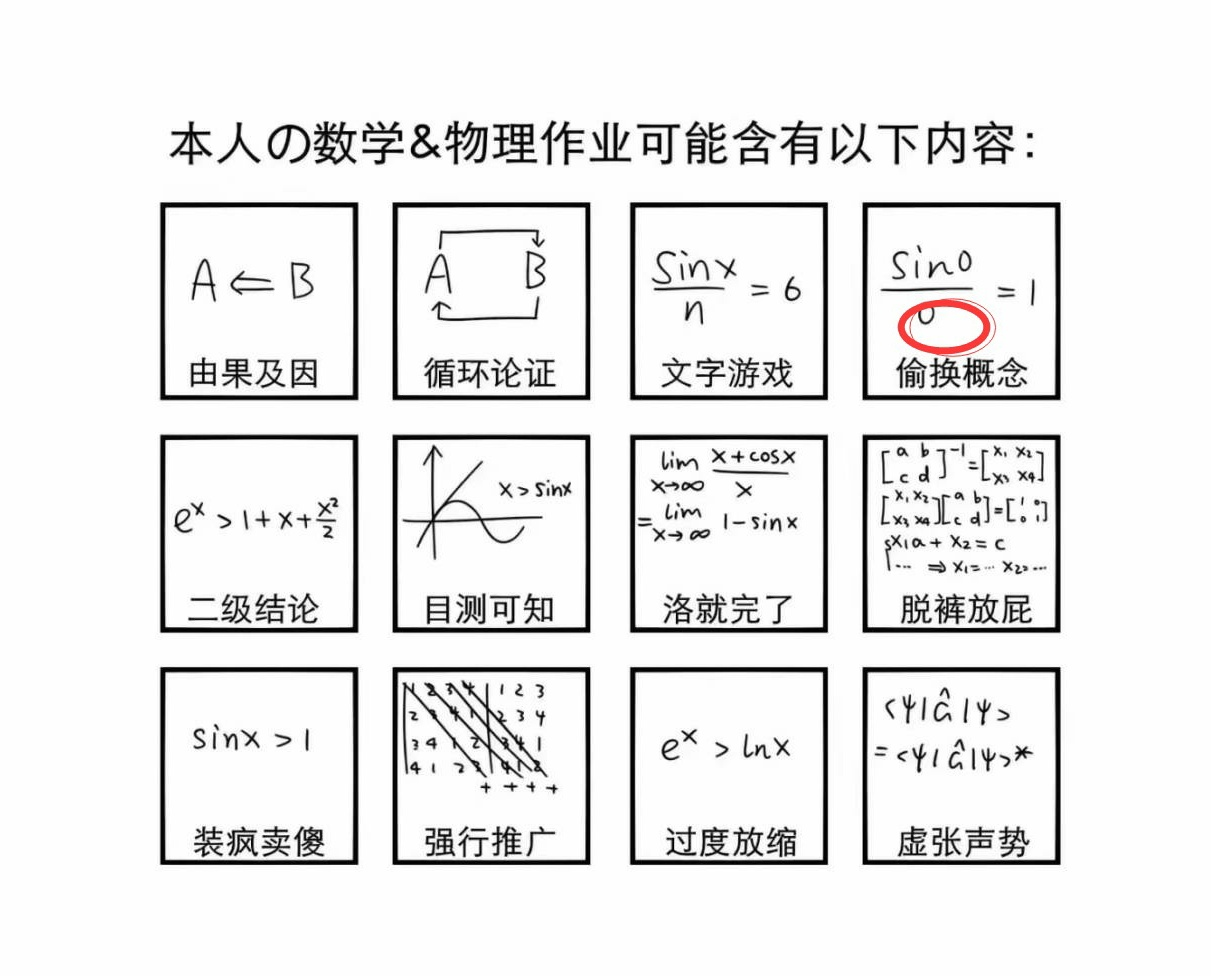
\includegraphics[width=6in]{Imgs/QQ_Image_1664445649724.jpg}
\end{figure}
\newpage




\begin{exercise}{1.2}
    如果$u:\R^3 \to \R$是关于$(x,y,z)$的函数
    \begin{gather*}
        \nabla f(u) = \frac{\dl f}{\dl u} \nabla u \\
        \nabla \cdot \bm{A}(u) = \nabla u \cdot \frac{\dl \bm{A}}{\dl u} \\
        \nabla \times \bm{A} (u) = \nabla u \times \frac{\dl \bm{A}}{\dl u}
    \end{gather*}
\end{exercise}
\begin{proof}
    \begin{align*}
        \nabla f(u) &= (\partial_{\mu} e^{\mu }) (f \circ u)(x) = \partial_{\mu} (f \circ u)(x) \e^{\mu} = \pp{f}{u} \pp{u}{x^{\mu}}\e^{\mu} = \frac{\dl f}{\dl u} \nabla u
    \end{align*}
    \begin{align*}
        \nabla \cdot \bm{A}(u) &= \partial_{\mu} A^{\mu} = \partial_{\mu} (A^{\mu} \circ u) (x) = \pp{A^{\mu}}{u} \pp{u}{x^{\mu}} = \frac{\dl \bm{A}}{\dl u} \cdot \nabla u
    \end{align*}
    \begin{align*}
        \nabla \times \bm{A} (u) &= \epsilon^{\mu \nu \rho} \nabla_{\mu} A_{\nu} \e_{\rho} = \epsilon^{\mu \nu \rho}  \partial_{\mu} (A_{\nu} \circ u)(x) \e_{\rho} = \epsilon^{\mu \nu \rho}  \pp{A_{\nu}}{u} \pp{u}{x^{\mu}} \e_{\rho} =\frac{\dl \bm{A}}{\dl u} \times \nabla u
    \end{align*}
\end{proof}


\begin{exercise}{1.3}
    设$\bm{r} = \bm{x} - \bm{x}',\; r = \sqrt{\sum_{i} (x^{i} - x'^{i})^2} $,定义$\nabla = \pp{}{x^{\mu}} \e^{\mu},\; \nabla ' = \pp{}{x'^{\mu}} \e^{\mu}$,证明
    \begin{gather*}
        \nabla r = -\nabla ' r = \frac{\bm{r}}{r} \\
        \nabla \frac{1}{r} = -\nabla' \frac{1}{r} = -\frac{\bm{r}}{r^3} \\
        \nabla \times \frac{\bm{r}}{r^3} = 0 \\
        \nabla \cdot \frac{\bm{r}}{r^3} = - \nabla' \cdot \frac{\bm{r}}{r^3} = 0 \\
    \end{gather*}
    同时求解$\nabla \cdot \bm{r},\; \nabla \times \bm{r},\; (\bm{a}\cdot \nabla)\bm{r},\; \nabla(\bm{a}\cdot \bm{r}),\; \nabla \cdot [E_0 \sin (\bm{k} \cdot \bm{r})],\; \nabla \times [E_0 \sin (\bm{k} \cdot \bm{r})]$
\end{exercise}
\begin{solution}
    易证$\partial_{\mu} \left( \dfrac{r_{\nu}}{r^3} \right) = \dfrac{\delta_{\mu \nu} r^2 - 3r_{\nu}r_{\mu}}{r^5},\; \partial_{\mu '} \left( \dfrac{r_{\nu}}{r^3} \right) = -\dfrac{\delta_{\mu \nu} r^2 - 3r_{\nu}r_{\mu}}{r^5}$,$\partial_{\mu} \dfrac{1}{r} = - \dfrac{r_{\mu}}{r^3}$\\
    (a) 
    \[
    \nabla r = \partial_{\mu} r \e^{\mu} = \frac{1}{r} r_{\mu} \e^{\mu} = \frac{\bm{r}}{r} 
    \]
    $\nabla' r$的结果是非常显然的。\\
    (b)
    \[
    \nabla \frac{1}{r} = \partial_{\mu} \frac{1}{r} \e^{\mu} = -\frac{1}{r^3} r_{\mu}\e^{\mu} = -\frac{\bm{r}}{r^3}
    \]
    (c)
    \begin{align*}
        \nabla \times \frac{\bm{r}}{r^3} &= \epsilon^{\mu \nu \rho} \partial_{\mu} \left( \frac{\bm{r}}{r^3} \right)_{\nu} \e_{\rho} = \frac{1}{r^5} \epsilon^{\mu \nu \rho} (\delta_{\mu \nu}r^2 - 3r_{\mu}r_{\nu})\e_{\rho} = \frac{-3}{r^5} \epsilon^{\mu \nu \rho} r_{\mu} r_{\nu} \e_{\rho}
    \end{align*}
   同时交换指标位置结果不变,即$\epsilon^{\mu \nu \rho} r_{\mu} r_{\nu} \e_{\rho} = \epsilon^{\nu \mu \rho} r_{\nu} r_{\mu} \e_{\rho}$,但只交换$\varepsilon$的指标会产生负值,即$\epsilon^{\nu \mu \rho} r_{\mu} r_{\nu} \e_{\rho} = - \epsilon^{\mu \nu \rho} r_{\mu} r_{\nu} \e_{\rho}$,观察到$\epsilon^{\nu \mu \rho} r_{\nu} r_{\mu} \e_{\rho} = - \epsilon^{\nu \mu \rho} r_{\mu} r_{\nu} \e_{\rho}$,由$\bm{r}$的任意性得$\epsilon^{\mu \nu \rho} = 0$.
    \[
      \nabla \times \frac{\bm{r}}{r^3} = 0
    \]
    (d)
    \begin{align*}
        \nabla \cdot \frac{\bm{r}}{r^3} = \partial_{\mu} \left( \frac{\bm{r}}{r^3} \right)^{\mu} = \frac{1}{r^5} ({\delta^{\mu}}_{\mu} r^2 - 3r^{\mu} r_{\mu}) =  \frac{1}{r^5} (3r^2 - 3r^2)=0
    \end{align*}
    (f)\\
    \[
        \nabla \cdot \bm{r} = 3
    \] 

    \[
        \nabla \times \bm{r} = \epsilon^{\mu \nu \rho} \partial_{\mu} r_{\nu} \e_{\rho} = \epsilon^{\mu \nu \rho} \delta_{\mu \nu} \e_{\rho} = 0
    \]

    \[
        (\bm{a} \cdot \nabla)\bm{r} = (a^{\mu} \partial_{\mu})\bm{r} = a^{\mu}\e_{\mu} = \bm{a}
    \]

    \[
        \nabla(\bm{a} \cdot \bm{r}) = (\partial_{\mu} \e^{\mu}) (a_{\nu} r^{\nu}) = a_{\nu}\partial_{\mu} r^{\nu} \e^{\mu} = a_{\nu}{\delta_{\mu}}^{\nu} \e^{\mu} = a_{\mu} \e^{\mu} = \bm{a}
    \]

    \begin{align*}
        \nabla \cdot [\bm{E}_0 \sin (\bm{k} \cdot \bm{r})] &= \partial_{\mu} \left[ (E_0)_{\mu} \sin (k_{\nu} r^{\nu}) \right] = (E_0)_{\mu} \cos (k_{\nu} r^{\nu}) k_{\mu} = [\bm{E}_0 \cos (\bm{k}\cdot \bm{r})] \cdot \bm{k}
    \end{align*}
    \begin{align*}
        \nabla \times [\bm{E}_0 \sin (\bm{k} \cdot \bm{r})] =  \epsilon^{\mu \nu \rho} \partial_{\mu} [(E_0)_{\nu} \sin (k_{a} r^a)] \e_{\rho} 
        = \epsilon^{\mu \nu \rho} (E_{0})_{\nu} \cos (k_a r^a) k_{\mu} \e_{\rho}
        = \bm{E}_0 \cos(\bm{k} \cdot \bm{r}) \times \bm{k}
    \end{align*}
\end{solution}






\begin{exercise}{1.5}
    若电荷系统的偶极矩定义为
    \[
    \bm{P}(t) = \int_{\mathcal{V}} \rho(\bm{r}', t) \bm{r}' \dl \tau'    
    \]
    利用$\nabla \cdot \bm{J} + \pp{\rho}{t} = 0$证明
    \[\pp{\bm{P}}{t} = \int_{\mathcal{V}} \bm{J}(\bm{r}',t)\dl \tau'\]
\end{exercise}
\begin{proof}
    \[
    \pp{\bm{P}}{t} = \int_{\mathcal{V}} \pp{\rho}{t}(\bm{r}', t) \bm{r}' \dl \tau' = \int_{\mathcal{V}} \pp{\rho}{t}(\bm{r}', t) x' \dl \tau' \e_x +  \int_{\mathcal{V}} \pp{\rho}{t}(\bm{r}', t) y' \dl \tau' \e_y +  \int_{\mathcal{V}} \pp{\rho}{t}(\bm{r}', t) z' \dl \tau' \e_z  
    \]
    只考察$x'$方向,有
    \begin{align*}
        \int_{\mathcal{V}} \pp{\rho}{t}(\bm{r}', t) x' \dl \tau' &= -\int_{\mathcal{V}} \nabla \cdot \bm{J} (\bm{r}', t) x' \dl \tau' \\
        &= -\int_{\mathcal{V}} \nabla \cdot (x'\bm{J} (\bm{r}', t)) - \nabla x' \cdot \bm{J} (\bm{r}', t) \dl \tau' \\
        &= -\oint_{\mathcal{S}} (x'\bm{J} (\bm{r}', t)) \cdot \dl \bm{a} + \int_{\mathcal{V}}\nabla x' \cdot \bm{J} (\bm{r}', t) \dl \tau'
    \end{align*}
    如果取$\mathcal{S} \to \infty$,由于边界处没有电流密度,故$\oint_{\mathcal{S}} (x'\bm{J} (\bm{r}', t)) \cdot \dl \bm{a} = 0$,另一方面$\nabla x' = (1, 0, 0)^{T}$,所以
    \[
        \int_{\mathcal{V}} \pp{\rho}{t}(\bm{r}', t) x' \dl \tau' = \int_{\mathcal{V}}J^{x} (\bm{r}', t) \dl \tau'
    \]
    从而得出
    \[
        \pp{\bm{P}}{t} = \int_{\mathcal{V}}\bm{J} (\bm{r}', t) \dl \tau'
    \]
\end{proof}





\begin{exercise}{1.6}
    $\bm{m}$是常矢量,定义矢量$\bm{A} = \dfrac{\bm{m} \times \bm{R}}{R^3}$,标量$\varphi = \dfrac{\bm{m} \cdot \bm{R}}{R^3}$,证明除$R= 0 $外有
    \[
    \nabla \times \bm{A} = -\nabla \varphi    
    \]
\end{exercise}
\begin{proof}
    $A_{\nu} = \epsilon_{ij \nu} m^{i} \dfrac{R^{j}}{R^3}$,$\nabla \times \bm{A} = \epsilon^{\mu \nu \rho} \partial_{\mu} A_{\nu} \e_{\rho}$,$\partial_i \left( \dfrac{R^{\mu}}{R^3}  \right) = \dfrac{{\delta^{\mu}}_i R^2 - 3R^{\mu}R_{i}}{R^5}$
    \begin{align*}
        \nabla \times \bm{A} &= \epsilon^{\mu \nu \rho} \partial_{\mu} \left(\epsilon_{ij \nu} m^{i} \dfrac{R^{j}}{R^3}\right) \e_{\rho} \\
         &= \epsilon^{\mu \nu \rho}\epsilon_{ij \nu} m^i \partial_{\mu} \left(\dfrac{R^{j}}{R^3}\right) \e_{\rho} \\
         &= \frac{1}{R^5} \epsilon^{\mu \nu \rho}\epsilon_{ij \nu} m^i ({\delta^{j}}_{\mu} R^2 - 3R^{j}R_{\mu}) \e_{\rho} \\
         &= \frac{1}{R^5} ({\delta^{\mu}}_{j}{\delta^{\rho}}_{i} - {\delta^{\mu}}_{i}{\delta^{\rho}}_{j}) ({\delta^{j}}_{\mu} R^2 - 3R^{j}R_{\mu}) m^i \e_{\rho} \\
         &= \frac{1}{R^5} \left[ {\delta^{\mu}}_{j}{\delta^{\rho}}_{i} {\delta^{j}}_{\mu} R^2 \e_{\rho} - 3 {\delta^{\mu}}_{j}{\delta^{\rho}}_{i} 3R^{j}R_{\mu} m^i \e_{\rho} - {\delta^{\mu}}_{i}{\delta^{\rho}}_{j}{\delta^{j}}_{\mu} R^2 \e_{\rho} + 3{\delta^{\mu}}_{i}{\delta^{\rho}}_{j} R^{j}R_{\mu} m^i \e_{\rho} \right]\\
         &= \frac{1}{R^5} \left[-3R^2 \bm{m}  + 3\bm{R} (\bm{R} \cdot \bm{m})\right]
    \end{align*}
    \begin{align*}
        -\nabla \varphi &= -\partial_{\mu} \left( m_i \frac{R^i}{R^3} \right) \e^{\mu} \\
        &= -\frac{1}{R^5} m_i ({\delta^i}_{\mu} R^2 - 3R^iR_{\mu})\e^{\mu} \\
        &= -\frac{1}{R^5} \left[ m_i {\delta^i}_{\mu} R^2 \e^{\mu} -  3 m_i R^iR_{\mu}\e^{\mu}  \right] \\
        &= -\frac{1}{R^5} \left[3R^2 \bm{m}  - 3\bm{R} (\bm{R} \cdot \bm{m})\right]
    \end{align*}
    % 先抄几个公式。
    % \begin{gather*}
    %     \nabla \times \frac{\bm{r}}{r^3} = 0 \\
    %     \nabla \cdot \frac{\bm{r}}{r^3} = 0 \\
    %     \nabla \times (\bm{u} \times \bm{v}) =  (\bm{v} \cdot \nabla) \bm{u} - (\nabla \cdot \bm{u}) \bm{v} + (\nabla \cdot \bm{v}) \bm{u} - (\bm{u} \cdot \nabla )\bm{v}
    % \end{gather*}
    % \begin{align*}
    %   \nabla \times \bm{A} &= \nabla \times \left(\bm{m} \times \dfrac{\bm{R}}{R^3} \right) \\
    %    &= \left( \dfrac{\bm{R}}{R^3} \cdot \nabla \right) \bm{m} - \left( \nabla \cdot \bm{m} \right)\dfrac{\bm{R}}{R^3} + \left( \nabla \cdot \dfrac{\bm{R}}{R^3} \right) \bm{m} - (\bm{u} \cdot \nabla) \dfrac{\bm{R}}{R^3} \\
    %    &= \left( \dfrac{R_{\mu}}{R^3} \partial_{\mu} \right) \bm{m} - \left( \partial_{\mu}m^{\mu} \right) \dfrac{\bm{R}}{R^3} + 0 \bm{m} - (\bm{u} \cdot \nabla) \dfrac{\bm{R}}{R^3} \\
    %    &=  - (\bm{u} \cdot \nabla) \dfrac{\bm{R}}{R^3}
    % \end{align*}
\end{proof}



\begin{exercise}{1.7}
    有一内外半径分别为$r_1, \; r_2$的空心介质球,介质电容率为$\varepsilon$,介质内均匀带静止自由电荷密度$\rho_f$,求\\
    (1)空间各点电场 \\
    (2)极化电荷和极化面电荷分布
\end{exercise}
\begin{solution}
    半径内包裹的电荷量
    \[
    Q(r) = (r^3 - r_1^3) \frac{4}{3} \pi \rho_f    
    \]
    \begin{itemize}
        \item $r_1 < r < r_2$时,由$\oint_{\mathcal{S}} \bm{D} \cdot \dl \bm{a} = Q(r)$得$D 4 \pi r^2 = (r^3 - r_1^3) \dfrac{4}{3} \pi \rho_f$;于是$D = \dfrac{r^3 - r_1^3}{3 r^2} \rho_f$。由$E = \dfrac{D}{\varepsilon}$得$E = \dfrac{r^3 - r_1^3}{3\varepsilon r^2} \rho_f$ .
        \item $r > r_2$时,$E = \dfrac{D}{\varepsilon_0}$,故$E = \dfrac{r_2^3 - r_1^3}{3\varepsilon_0 r_2^2} \rho_f$.
        \item $r < r_1$时,由于$Q =0 $,故$D = 0$,得$E = 0$。
    \end{itemize}
    边界处
    \[
    (\bm{P}_2 - \bm{P}_1)\cdot \e_n = -\sigma_P    
    \]
    成立,区别于电荷密度$\rho$,电荷面密度用$\sigma$表示。另外$\bm{P} = \chi_e \varepsilon_0 \bm{E} \Rightarrow \bm{P} = (\varepsilon_0 - \varepsilon)\bm{E}$,$\bm{P}$与$\bm{E}$共线时有$P = (\varepsilon_0 - \varepsilon)E$.
    \begin{itemize}
        \item $r_2$面上,$P_2 = 0,\; P_1 = (\varepsilon - \varepsilon_0)E_1 = (\varepsilon - \varepsilon_0)\dfrac{r_2^3 - r_1^3}{3\varepsilon r_2^2} \rho_f$,因此$\sigma_P = (\varepsilon - \varepsilon_0)\dfrac{r_2^3 - r_1^3}{3\varepsilon r_2^2} \rho_f$.
        \item $r_1$面上,$P_0 = 0$,$P_1= (\varepsilon - \varepsilon_0)(\varepsilon - \varepsilon_0)\dfrac{r_1^3 - r_1^3}{3\varepsilon r_1^2} \rho_f = 0$,所以$\sigma_P = 0$.
    \end{itemize}
\end{solution}






\begin{exercise}{1.8}
    内外i半径分别为$r_1,\; r_2$的中空导体圆柱,沿着轴向有恒定均匀自由电流$\bm{J}_f$,导体内磁导率为$\mu$,求磁感应强度和磁化电流。
\end{exercise}
\begin{solution}
    由$\oint_{L} \bm{H} \cdot \dl \bm{l} = I_f + \int_{\mathcal{S}} \pp{\bm{D}}{t} \dl \bm{a}$,以及$\pp{\bm{D}}{t} = 0$得$\oint_{L} \bm{H} \cdot \dl \bm{l} = I_f$.
    \begin{itemize}
        \item $r_1 < r < r_2$时,$\oint_{L} \bm{H} \cdot \dl \bm{l} = H 2 \pi r = (\pi r_2^2 - \pi r_1^2) J_f \dfrac{\pi r^2 - \pi r_1^2}{\pi r_2^2 - \pi r_1^2}$,得出$H = \dfrac{(r^2 - r_1^2) J_f}{2r}$。目测可知$\bm{H}$的方向是$\bm{J} \times \bm{r}$的方向,所以上式左右分别乘$\hbm{H},\;\hbm{J} \times \hbm{r}$,得$\bm{H} = \dfrac{(r^2 - r_1^2) \bm{J}_f \times \bm{r}}{2r^2}$,再用$\bm{B} = \mu \bm{H}$得$\bm{B} = \dfrac{\mu (r^2 - r_1^2) \bm{J}_f \times \bm{r}}{2r^2}$.
        \item $r > r_2$时,$H = \dfrac{(r_2^2 - r_1^2) J_f}{2r}$,即得$\bm{H} = \dfrac{(r_2^2 - r_1^2) \bm{J}_f \times \bm{r}}{2r^2}$,$\bm{B} = \dfrac{\mu (r_2^2 - r_1^2) \bm{J}_f \times \bm{r}}{2r^2}$.
        \item $r <r_1$时,$J = 0$,故$\bm{B} = 0$.
    \end{itemize}
    在边界处取一高度不太高的截面,切向方向为$\Delta \bm{l}$,通过该截面的磁化电流为(P.27.(5.9)).
    \[
    I_M = (\e_n \times \Delta \bm{l}) \cdot \bm{a}_M    
    \]
    为了区别电流密度与电流线密度,用$a$表示电流线密度。
    \[
        (\bm{M}_2 - \bm{M}_1) \cdot \Delta \bm{l} = I_M = (\e_n \times \Delta \bm{l}) \cdot \bm{a}_M = (\bm{a}_M \times \e_n)\cdot \Delta \bm{l}
    \]
    $ (\bm{M}_2 - \bm{M}_1) = (\bm{a}_M \times \e_n)$两端同时叉乘$\e_n$,利用123=213-312公式以及$\e_n$与$\bm{a}_M$正交;得到$\boxed{\e_n \times (\bm{M}_2 - \bm{M}_1) = \bm{a}_M}$.
    \begin{itemize}
        \item $r_2$面上,$\bm{M}_2 = 0$,所以$- \e_n \times \bm{M}_1 = \bm{a}_M$;同时$\bm{M}_1 = \chi_M \bm{H}_1 = \left( \dfrac{\mu}{\mu_0} - 1\right) \bm{H}_1 $,可见$\bm{a}_M = \left( \dfrac{\mu}{\mu_0} - 1\right) \e_n \times \bm{H}_1$,$\e_n$与$\bm{r}$方向一致。
    \end{itemize}
    \begin{align*}
        \left( \dfrac{\mu}{\mu_0} - 1\right) \e_n \times \bm{H}_1 &= \left( \dfrac{\mu}{\mu_0} - 1\right) \left[ \e_n \times \left( \frac{1}{2} \bm{J}_f \times \bm{r} - \frac{r_1^2}{2r^2} \bm{J}_f \times \bm{r} \right) \right]_{r=r_2} \\
        &= \left( \dfrac{\mu}{\mu_0} - 1\right) \left[ \frac{r^2 - r_1^2}{2r} \right]_{r=r_2} J_f \\
        &= \left( \dfrac{\mu}{\mu_0} - 1\right) \frac{r_2^2 - r_1^2}{2r_2} J_f
    \end{align*}
    \begin{itemize}
        \item $r_1$面上,$\bm{M}_0 = 0$,所以$\e_n \times \bm{M}_1 = \bm{a}_M$,借用上面的推倒得到$\bm{a}_M =  \left( \dfrac{\mu}{\mu_0} - 1\right) \dfrac{r_1^2 - r_1^2}{2r_1} J_f = 0$.
        \item $r_1 < r < r_2$,利用$\dfrac{1}{\mu_0} \nabla \times \bm{B} = \bm{J}_f + \bm{J}_M + \bm{J}_P + \varepsilon_0 \pp{\bm{E}}{t}$,得到$\dfrac{1}{\mu_0} \nabla \times \bm{B} - \bm{J}_f = \bm{J}_M$,最终得$\bm{J}_M = \left( \dfrac{\mu}{\mu_0} - 1 \right) \bm{J}_f$
    \end{itemize}
    \begin{align*}
        \nabla \times \bm{B} &= \nabla \times \left[\dfrac{\mu (r^2 - r_1^2) \bm{J}_f \times \bm{r}}{2r^2} \right] \\
        &= \frac{\mu}{2} \nabla \times (\bm{J}_f \times \bm{r}) - \frac{\mu r_1^2 }{2} \nabla \times (\bm{J} \times \frac{\bm{r}}{r^2}) \\
        &= \frac{\mu}{2} \left[ (\bm{r} \cdot \nabla)\bm{J}_f - (\nabla \cdot \bm{J}_f) \bm{r} + (\nabla \cdot \bm{r})\bm{J}_f - (\bm{J}_f \cdot \nabla)\bm{r} \right] \\
        &- \frac{\mu r_1^2}{2} \left[ (\frac{\bm{r}}{r^2} \cdot \nabla)\bm{J}_f - (\nabla \cdot \bm{J}_f) \frac{\bm{r}}{r^2} + (\nabla \cdot \frac{\bm{r}}{r^2})\bm{J}_f - (\bm{J}_f \cdot \nabla)\frac{\bm{r}}{r^2} \right] \\
        &= \frac{\mu}{2} \left[ 0-0+3\bm{J}_f - \bm{J}_f \right] - \frac{\mu r_1^2}{2} \left[ 0-0+\frac{1}{r^2}\bm{J}_f - \frac{1}{r^2}\bm{J}_f \right] \\
        &= \mu \bm{J}_f
    \end{align*}
\end{solution}





\begin{exercise}{1.9}
    证明均匀介质内部的极化电荷密度总是满足$\rho_P = -\left( 1 - \dfrac{\varepsilon_0}{\varepsilon} \right) \rho_f$.
\end{exercise}
\begin{proof}
    首先从$\nabla \cdot (\varepsilon_0 \bm{E} + \bm{P}) = \rho_f$得出$\rho_P = \varepsilon_0 \nabla \cdot \bm{E} - \rho_f $.再者,利用$\bm{P} = \chi_e \varepsilon_0 \bm{E} = (\varepsilon - \varepsilon_0) \bm{E} $得到$-\rho_P = \nabla \cdot \bm{P} = (\varepsilon - \varepsilon_0) \nabla \cdot \bm{E}$.联立两个方程
    \[
    \left\{
        \begin{aligned}
            & \rho_P = \varepsilon_0 \nabla \cdot \bm{E} - \rho_f \\
            & \rho_P = -(\varepsilon - \varepsilon_0) \nabla \cdot \bm{E}
        \end{aligned} 
    \right.    
    \]
    解得$\rho_P = -\left( 1 - \dfrac{\varepsilon_0}{\varepsilon} \right) \rho_f$.
\end{proof}





\begin{exercise}{1.10}
    证明两个闭合的恒定电流圈之间的相互作用力大小相等,方向相反。
\end{exercise}
\begin{proof}
    定义光滑环闭道路$\Gamma_a :I_a \to \R^3,\; \Gamma_b : I_b \to \R^3$,其像点分别表示为$\Gamma_a,\; \Gamma_b$,稳定电流分别表示为$I_a,\; I_b$,参数分别使用$t, \tau$。根据$\bm{B}(\bm{r}) = \dfrac{\mu_0}{4 \pi} \int_{\mathcal{V}} \dfrac{\bm{J}(\bm{r}') \times \bm{\imath}}{\imath^3} \dl \tau'$,得出道路$\Gamma_a$在$\Gamma_b$上一点的磁感应强度为
    \[
    \bm{B}_{ab}(\tau) = \frac{\mu_0I_a}{4\pi} \oint\limits_{\Gamma_a} \frac{1}{\vert \Gamma_b(\tau) - \Gamma_a(t)\vert ^3} \dot{\Gamma}_a(t) \times (\Gamma_b(\tau) - \Gamma_a(t)) \dl t 
    \]
    其中$\dot{\Gamma}_a(t) = ((\dot{\Gamma}_a)^1, (\dot{\Gamma}_a)^2, (\dot{\Gamma}_a)^3) (t)$,为了方便,后文用$A(t),\; B(\tau)$代替$\Gamma_a(t),\; \Gamma_b(\tau)$,用$a(t),\; b(\tau)$代替$\dot{\Gamma}_a(t),\; \dot{\Gamma}_b(\tau)$,于是
    \begin{gather*}
        B_{ab}(\tau) = \frac{\mu_0I_a}{4\pi} \oint\limits_{\Gamma_a} \frac{1}{\vert B - A \vert ^3} a \times (B - A) \dl t  \\
        B_{ba}(t) =\frac{\mu_0I_b}{4\pi}  \oint\limits_{\Gamma_b} \frac{1}{\vert A - B \vert ^3} b \times (A - B) \dl \tau
    \end{gather*} 
    考察$\Gamma_b$的受力情况
    \[
    F_{ab} = \oint\limits_{\Gamma _b} B_{ab}(\tau) \times (I_b \dl l_b) =  I_b \oint\limits_{\Gamma _b}  B_{ab}(\tau) \times b(\tau) \dl \tau
    \]
    展开后得到
    \begin{align*}
    F_{ab} &= \frac{\mu_0 I_a I_b}{4\pi} \oint\limits_{\Gamma _b} \oint\limits_{\Gamma_a} \frac{1}{\vert B - A \vert ^3} \epsilon^{\mu \nu \rho} \epsilon_{ij\mu} a^i (B^j - A^j)b_{\nu} \e_{\rho} \dl t \dl \tau \\
    &= \frac{\mu_0 I_a I_b}{4\pi} \oint\limits_{\Gamma _b} \oint\limits_{\Gamma_a} \frac{1}{\vert B - A \vert ^3} ({\delta^{\nu}}_i{\delta^{\rho}}_j - {\delta^{\nu}}_j{\delta^{\rho}}_i) a^i (B^j - A^j)b_{\nu} \e_{\rho} \dl t\dl \tau \\
    &= \frac{\mu_0 I_a I_b}{4\pi} \oint\limits_{\Gamma _b} \oint\limits_{\Gamma_a} \frac{1}{\vert B - A \vert ^3} (a^{\nu}A^{\rho}b_{\nu}\e_{rho} - a^{\nu} A^{\rho} b_{\nu} \e_{\rho} - a^{\rho}B^{\nu}b_{\nu}\e_{\rho} + a^{\rho} A^{\nu} b_{nu} \e_{\rho}) \dl t \dl \tau \\
    % &= \frac{\mu_0 I_a I_b}{4\pi} \left[ \oint\limits_{\Gamma _b} \oint\limits_{\Gamma_a} \frac{(a \cdot B)(B-A)}{\vert B - A \vert ^3}  \dl t \dl \tau - \oint\limits_{\Gamma _b} \oint\limits_{\Gamma_a}  \frac{b\cdot (B-A)}{\vert B - A \vert ^3} a \dl t \dl \tau\right] \\
    &=  \frac{\mu_0 I_a I_b}{4\pi} \left[ \oint\limits_{\Gamma _b} \oint\limits_{\Gamma_a} \frac{(a \cdot b)(B-A)}{\vert B - A \vert ^3}  \dl t \dl \tau - \oint\limits_{\Gamma _a} \oint\limits_{\Gamma_b}  \frac{(B-A)}{\vert B - A \vert ^3}\cdot \dl B \dl A\right] \\
    &=  \frac{\mu_0 I_a I_b}{4\pi}\oint\limits_{\Gamma _b} \oint\limits_{\Gamma_a} \frac{(a \cdot b)(B-A)}{\vert B - A \vert ^3}  \dl t \dl \tau
    \end{align*}
    % 由于$\oint\limits_{\Gamma_b}  \dfrac{(B-A)}{\vert B - A \vert ^3}\cdot \dl B = \int_{\mathcal{S}_b} \nabla \times \dfrac{(B-A)}{\vert B - A \vert ^3} \cdot \dl S_b$
    同样,考察$\Gamma_a$的受力情况,得到
    \[
        F_{ba} = -\frac{\mu_0 I_a I_b}{4\pi}\oint\limits_{\Gamma _b} \oint\limits_{\Gamma_a} \frac{(a \cdot b)(B-A)}{\vert B - A \vert ^3}  \dl t \dl \tau
    \]
\end{proof}







\begin{exercise}{1.11}
    平行板电容器有两层介质,厚度分别为$l_1, l_2$,电容率为$\varepsilon_1,\; \varepsilon_2$,在两板接上电动势为$\xi$的电池 \\
    (1)电容器两板上的自由电荷面密度$\omega_f$\\
    (2)介质分界面上的自由电荷面密度$\omega_f$ \\
    (3)若介质漏电,电导率为$\sigma_1,\; \sigma_2$,电流达到恒定时,上述结果如何?
\end{exercise}
\begin{solution}
    \quad \\
    (1)由$\e_n \cdot (\bm{D}_2 - \bm{D}_1) = \sigma_f$得,极板1上满足$D_1 - D_{10} = \omega_{f_1}$,极板2上满足$D_{20} - D_2 = \omega_{f_2}$,介质分界面不存在自由电荷,所以$D_2 - D_1 = \omega_{f_3} = 0$. 同时由$\bm{D} = \varepsilon \bm{E}$, 得下述方程
    \[
    \left\{
        \begin{aligned}
            & \varepsilon_1 E_1 = \omega_{f_1} \\
            & \varepsilon_2 E_2 = -\omega_{f_2} \\
            & E_1 l_1 + E_2 l_2 = \xi \\
            &  \varepsilon_1 E_1 - \varepsilon_2 E_2 = 0
        \end{aligned}
    \right.    
    \]
    解得$E_1 = \dfrac{\varepsilon_2 \xi}{\varepsilon_2l_1 + \varepsilon_1l_2}, \; E_2 = \dfrac{\varepsilon_1 \xi}{\varepsilon_2l_1 + \varepsilon_1l_2},\; \omega_{f_1} = \dfrac{\varepsilon_1 \varepsilon_2 \xi}{\varepsilon_2l_1 + \varepsilon_1l_2},\; \omega_{f_2} = -\dfrac{\varepsilon_1 \varepsilon_2 \xi}{\varepsilon_2l_1 + \varepsilon_1l_2},\; \omega_{f_3} = 0$.\\
    (2)根据欧姆定律$\bm{J} = \sigma \bm{E}$,以及介质电流恒定,得$J = \sigma_1 E_1 = \sigma_2 E_2$,求解下述方程组
    \[
    \left\{
        \begin{aligned}
            & E_1 l_1 + E_2 l_2 = \xi \\
            &  \omega_1 E_1 = \omega_2 E_2\\ 
            & \varepsilon_1 E_1 = \omega_{f_1} \\
            & \varepsilon_2 E_2 = -\omega_{f_2} \\
            &  \varepsilon_2 E_2 -  \varepsilon_1 E_1 = \omega_{f_3}
        \end{aligned}
    \right.    
    \]
    解得$E_1 = \dfrac{\sigma_2 \xi}{\varepsilon_2l_1 + \varepsilon_1l_2},\; E_2 = \dfrac{\sigma_1 \xi}{\varepsilon_2l_1 + \varepsilon_1l_2},\; \omega_{f_1} = \dfrac{\varepsilon_1 \sigma_2 \xi}{\varepsilon_2l_1 + \varepsilon_1l_2},\; \omega_{f_2} = \dfrac{\varepsilon_2 \sigma_1 \xi}{\varepsilon_2l_1 + \varepsilon_1l_2}$ .\\
    $\omega_{f_3} = \dfrac{\varepsilon_2 \sigma_1 \xi}{\varepsilon_2l_1 + \varepsilon_1l_2} - \dfrac{\varepsilon_1 \sigma_2 \xi}{\varepsilon_2l_1 + \varepsilon_1l_2}$.
\end{solution}































\end{document}